\chapter[Aula 10]{Medida Produto e o Teorema de Fubini}
\chaptermark{}

\section{Espaço Produto}

Considere $(X, \mathscr{X})$ e $(Y, \mathscr{Y})$ espaços mensuráveis. 
Já que o produto cartesiano de $\sigma$-álgebras não 
é necessariamente uma $\sigma$-álgebra, 
a construção mais simples que nos resta é 
considerar em $X\times Y$ a $\sigma$-álgebra gerada pelos
{\it retângulos mensuráveis}, isto é, a $\sigma$-álgebra gerada
pela coleção 
$\mathscr{R}=\{ A\times B:\ A\in \mathscr{X}, B\in \mathscr{Y}\}.$ 
A $\sigma$-álgebra gerada por $\mathscr{R}$ 
é conhecida como $\sigma$-álgebra produto e 
usamos a seguinte notação $\mathscr{X}\times \mathscr{Y}$
para nos referirmos a esta $\sigma$-álgebra.



\begin{proposicao}\label{Prod. 1}
Sejam $(X, \mathscr{X})$ e $(Y, \mathscr{Y})$ espaços mensuráveis e 
$\mathscr{X}\times \mathscr{Y}$ a sigma-álgebra produto em $X\times Y$.
Então as seguintes afirmações são verdadeiras:
\begin{itemize}
\item[a)] Se $E\in \mathscr{X}\times \mathscr{Y}$ então, para cada $x\in X$ fixado,
o conjunto $[y: (x,y)\in E]:=\{y\in Y: (x,y)\in E\}$ é $\mathscr{Y}$-mensurável. 
De modo análogo, fixado $y\in Y$, 
o conjunto $[x:(x,y)\in E]:=\{x\in X: (x,y)\in E\}$ 
é $\mathscr{X}$-mensurável.



\item[b)] Se $f:X\times Y\to \mathbb{R}$ é uma função $\mathscr{X}\times \mathscr{Y}$ mensurável 
então, para cada $x\in X$ fixado, a função $y\mapsto f(x,y)$ é $\mathscr{Y}$-mensurável. De 
modo análogo, para cada $y\in Y$ fixo, a função $x\mapsto f(x,y)$ é $\mathscr{X}$-mensurável.
\end{itemize}
\end{proposicao}


\begin{proof}
\emph{Prova do item a)}. Fixe $x\in X$ e considere a aplicação  
$T_x:Y\to X\times Y$ dada por $T_x(y)=(x,y)$.
Note que se $E=A\times B\in \mathscr{X}\times \mathscr{Y}$
é um retângulo mensurável então $T_{x}^{-1}E=B~\textnormal{ou}~\varnothing$ 
dependendo apenas se 
$A$ contém ou não o ponto $x$.  
\begin{figure}
\centering
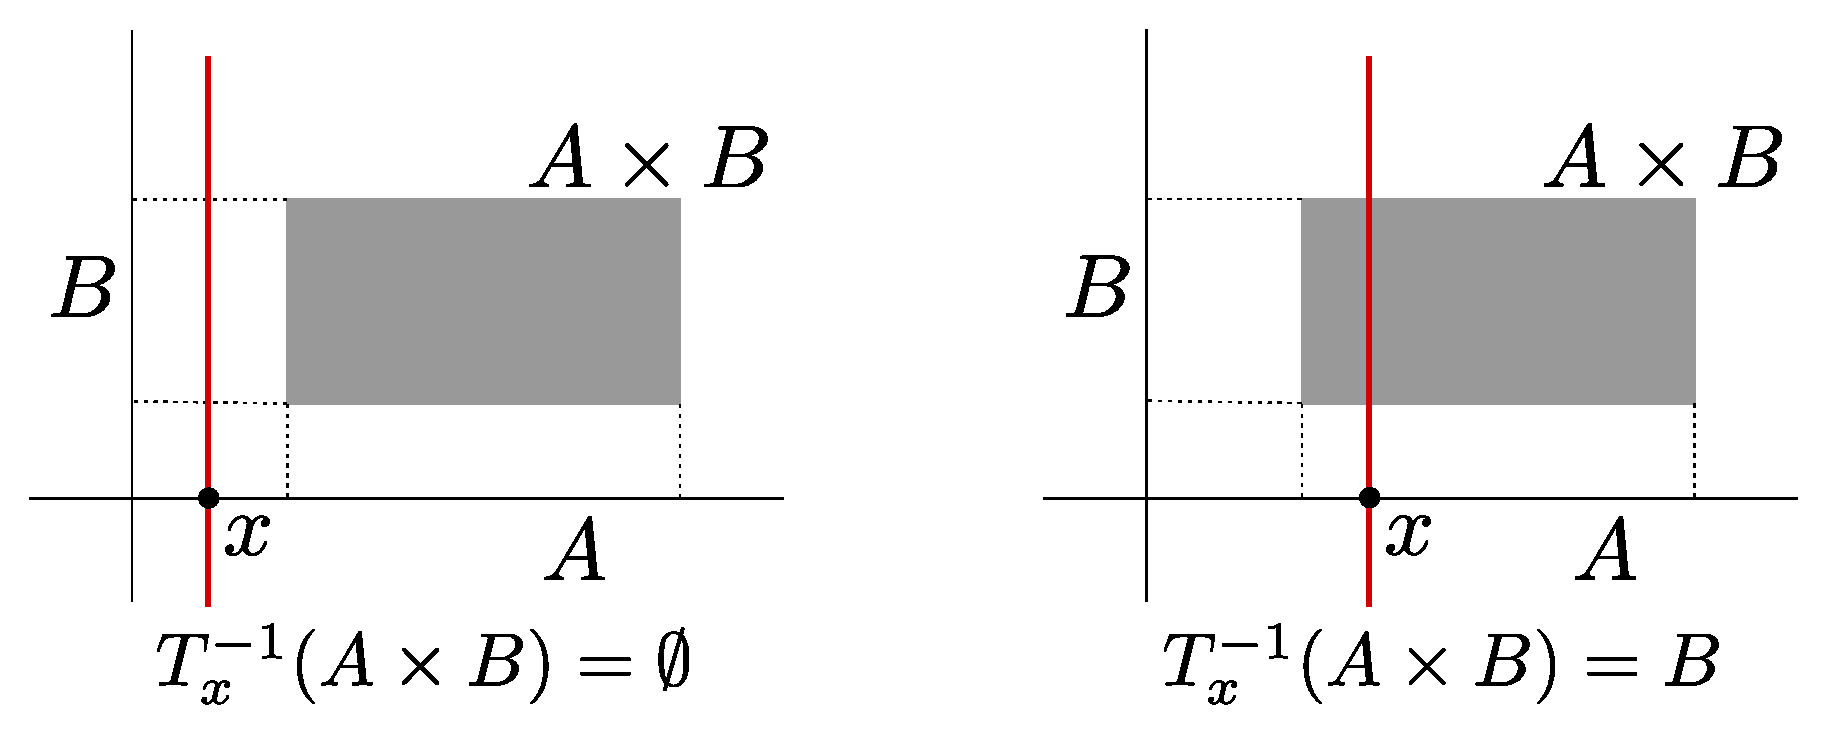
\includegraphics[scale=0.3]{Figuras/fig-medida-produto-aula10}
\caption{}
\label{medida-produto-1}
\end{figure}

\newpage
De qualquer forma 
em ambas situações temos que $T_x^{-1}E\in \mathscr{Y}$.
Para mostrar que a afirmação também é válida para um conjunto 
$E$ arbitrário de $\mathscr{X}\times \mathscr{Y}$, 
basta notar que $[y: (x,y)\in E] = T^{-1}_{x}(E)$ e 
usar o seguinte exercício
\begin{exercicio}
	Sejam $(\Omega',\mathcal{F}')$ e $(\Omega,\mathcal{F})$
	dois espaços mensuráveis e $T:\Omega'\to\Omega$ uma função. 
	Suponha que $\mathcal{F}= \sigma(\mathscr{R})$
	para alguma coleção $\mathscr{R}$ de subconjuntos de $\Omega$.
	Se para todo $R\in \mathscr{R}$ temos $T^{-1}(R)\in \mathcal{F}'$
	então $T^{-1}(E)\in \mathcal{F}'$ para todo $E\in \mathcal{F}$.
\end{exercicio}
%
A prova de que $[x: (x,y)\in E]$ é $\mathscr{X}$-mensurável é feita de 
forma completamente análoga considerando a aplicação 
$T_y:X\to X\times Y$, dada por $T_y(x)=(x,y)$.

\bigskip
\noindent \emph{Prova do item b)}.  
Fixado $x\in X$ podemos observar que a aplicação $y\mapsto f(x,y)$
é dada por $f\circ T_{x}$, onde $T_x:Y\to X\times Y$ é a aplicação 
definida na prova do item a). Já que $f$ é $\mathscr{X}\times\mathscr{Y}$-mensurável
temos do item a) para qualquer boreliano $B\in \mathscr{B}(\mathbb{R})$ que 
$(f\circ T_x)^{-1}(B)= T^{-1}_x(f^{-1}(B)) \in \mathscr{Y}$.
Mostrando que $y\mapsto f(x,y)$ é $\mathscr{Y}$-mensurável para qualquer 
$x\in X$ fixado. A prova de que $x\mapsto f(x,y)$ é $\mathscr{X}$-mensurável 
para qualquer $y\in Y$ fixado é feita de maneira análoga.
\end{proof}


\begin{observacao}
Os conjunto $[y: (x,y)\in E]$ e $[x: (x,y)\in E]$ 
são chamados de seções de $E$ determinadas por $x$ e 
por $y$, respectivamente. Do mesmo modo as funções $f(x, \cdot)$ e $f(\cdot, y)$ 
são chamadas as seções de $f$ determinadas por $x$ e por $y$ respectivamente.
\end{observacao}



\section{Medidas Produto}
Sejam $(X, \mathscr{X}, \mu)$ e $(Y, \mathscr{Y}, \nu)$
 espaços de medida. A nossa  vontade é encontrar uma medida $\pi$ definida 
 em $\mathscr{X}\times \mathscr{Y}$ tal que se $E=A\times B$ seja um retângulo mensurável 
 tenhamos que $\pi(E)=\mu(A)\nu(B)$. A seguir vamos ver que quando 
 $ \mu$ e $\nu$ são sigma finitas a \emph{medida produto} não só existe como é única.
 \medskip
 

Sejam $(X, \mathscr{X}, \mu)$ e $(Y, \mathscr{Y}, \nu)$
 espaços de medida com $\mu$ e $\nu$ finitas. 
 Temos pela proposição (\ref{Prod. 1}) que dado
  $E\in \mathscr{X}\times \mathscr{Y}$ as funções 
  $X\ni x\mapsto \nu(E_x)\in [0, \infty)$ e
   $Y\ni y\mapsto \mu(E_y)\in [0, \infty)$ estão bem definidas.
Denote por $\mathscr{L}$ a classe dos $E\in \mathscr{X}\times \mathscr{Y}$
para os quais as funções acima são $\mathscr{X}$ e $\mathscr{Y}$ mensuráveis 
respectivamente.

\begin{proposicao}\label{Mens. Prod}
A classe $\mathscr{L}$ coincide com $\mathscr{X}\times \mathscr{Y}$.
\end{proposicao}
\begin{proof}
Começamos por mostrar que $\mathscr{L}$ é um $\lambda$-sistema. De fato, temos que
$\nu_x(X\times Y)=\nu(Y) < \infty$ para todo $x\in X$ e, portanto
 a função $X\ni x\mapsto \nu_x(X\times Y)\in [0,\infty)$ é claramente mensurável.
  Agora note que $\nu_x(E^c)=\nu(E^c_x)=\nu((E_x)^c)=1-\nu(E_x).$
 Assim, se $X\ni x\mapsto \nu_x(E)\in [0, \infty)$  é mensurável temos que 
 $X\ni x\mapsto \nu_x(E^c)=1-\nu_x(E)\in [0, \infty)$ é mensurável, sendo pois 
 a diferença de duas funções mensuráveis.
  Sejam $E_1, E_2, \ldots E_n, \ldots$ conjuntos em $\mathscr{L}.$ É suficiente 
  considerarmos o caso em que os $E_n^{'s}$ são disjuntos.
  Note que $E_x=(\bigcup E_n)_x=\bigcup (E_n)_x$. Assim temos que 
  $$
  \nu_x(E)=\nu(E_x)=\nu(\bigcup (E_n)_x)=\sum_{n\geq 1}\nu_x(E_n).
  $$
  Como, por hipótese, para cada $n$, o mapa $X\ni x\mapsto \nu_x(E_n)\in [0,\infty)$ é mensurável, segue que 
  o mapa 
  $$
 X\ni x\mapsto \nu_x(E)=\sum_{n\geq 1}\nu_x(E_n)\in [0,\infty),
 $$ 
 pois a medida $\nu$ é $\sigma$-finita. Como esse mapa é o 
limite de uma sequência de funções mensuráveis, ele também será mensurável. Isto conclui que $\mathscr{L}$ é um $\lambda$-sistema.
 
 Para finalizar veja  que $\mathscr{L}$ contém os retângulos mensuráveis $\mathscr{R}$, com efeito se $E=A\times B\in \mathscr{R}$ então o mapa $x\mapsto \nu(E_x)$ pode ser escrito como $1_A(x)\nu(B)$ que é claramente mensurável. Sendo assim temos pelo Teorema $\pi$-$\lambda$ que $\mathscr{X}\times \mathscr{Y}= \sigma(\mathscr{R})\subset \mathscr{L}\subset \mathscr{X}\times \mathscr{Y}$ concluindo a demonstração.
\end{proof}
\medskip


Passemos à construção da medida produto. Comecemos definindo funções de conjunto $\pi_1$ e $\pi_2$ como segue
\begin{equation}\label{M.Prod. 1}
\pi_1(E)=\int_X \nu_x(E) d\mu(x),~~~~~E \in \mathscr{X}\times \mathscr{Y}
\end{equation}
e 
\begin{equation}\label{M. Prod. 2}
\pi_2(E)=\int_Y \mu_y(E)d\nu(y),~~~~~E \in \mathscr{X}\times \mathscr{Y}
\end{equation}
é fácil ver que tanto $\pi_1$ quanto $\pi_2$ são medidas finitas em $\mathscr{X}\times \mathscr{Y}$. Agora note que se $E=A\times B\in\mathscr{X}\times \mathscr{Y}$  é um retângulo mensurável então temos que  $\nu_x(E)=1_A(x)\nu(B)$ e $\mu_y(E)=1_B\mu(A)$, de modo que 
\begin{equation}
\pi_1(A\times B)=\mu(A)\nu(B)=\pi_2(A\times B)
\end{equation}
de modo que as medidas $\pi_1$ e $\pi_2$ coincidem no $\pi$-sistema $\mathscr{R}$.  Denote por $\mathscr{L}$ a classe dos elementos $E$ de 
$\mathscr{X}\times \mathscr{Y}$  para os quais $\pi_1(E)=\pi_2(E)$.

\begin{proposicao}
A classe $\mathscr{L}$ coincide com $\mathscr{X}\times \mathscr{Y}$
\end{proposicao}


\begin{proof}
Seja $E=X\times Y$, então $\nu_x(E)=1_X(x)\nu(Y)=1_X(x)$ e $\mu_y(E)=1_Y(y)\mu(X)=1_Y(y)$. Portanto 
$$
\pi_1(X\times Y)=1=\pi_2(X\times Y)
$$
donde $X\times Y\in \mathscr{L}$. Seja $E\in \mathscr{L}$, então temos que
$$
\begin{array}{rcl}
\pi_1(E^c)&=&\displaystyle\int_X \nu_x(E^c)d\mu(x)
=
\int_X (1-\nu_x(E))d\mu(x)
\\[5mm]
&
=
&
\displaystyle 1-\int_X\nu_x(E) d\mu (x)
=
1-\int_Y \mu_y(E)d\nu(y)
\\[5mm]
&
=
&
1-\pi_2(E)
\\[5mm]
&
=
&
\pi_2(E^c)
\end{array}
$$
portanto $E^c\in \mathscr{L}$.  
Finalmente sejam $E_1, \ldots, E_n, \ldots $ em $\mathscr{L}$, vamos
mostrar que $E=\bigcup E_n\in \mathscr{L}.$ É suficiente considerar
o caso em que os $E_n^{'s}$ são disjuntos. Para cada $n$ considere os
conjunto $\bigcup_{j=1}^nE_n$, é claro que   $\bigcup_{j=1}^nE_n\nearrow E.$ Note
também que para cada $n$ a função $x\mapsto \nu_x(E_n)$ é uma função não negativa.
Sendo assim a temos que  $f_n=\sum_{j=1}^n\nu_{(\cdot)}(E_j)=\nu_x(\bigcup_{j=1}^{n}E_j)$
e $g_n=\sum_{j=1}^n\mu_{(\cdot)}(E_j)=\mu_y(\bigcup_{j=1}^{n}E_j)$ são
uma famílias não decrescentes de funções não negativas.
Portanto segue do teorema da convergência monótona
que
$$
\begin{array}{rcl}
\pi_1(E)&=&\displaystyle\lim_{n\to \infty}\pi_1(\bigcup_{j=1}^{n}E_j)
=
\lim_{n\to \infty}\int_X \nu_x(\bigcup_{j=1}^{n}E_j))d\mu(x)
\\[5mm]
&
=
&
\displaystyle \lim_{n\to \infty}\int_X (\sum_{j=1}^n\nu_x(E_j)) d\mu(x)
=
\lim_{n\to \infty}\int_Y(\sum_{j=1}^{n}\mu_y(E_j)d\nu(y)
\\[5mm]
&
=
&
\displaystyle\lim_{n\to \infty} \int_Y \mu_y(\bigcup_{j=1}^{n}E_j)d\nu(y)
\\
&=&
\pi_2(E)
\end{array}
$$
concluindo que $E\in \mathscr{L}$. Portanto $\mathscr{L}$ é um $\lambda$-sistema 
que contém o $\pi$-sistema $\mathscr{R}$, logo $\mathscr{X}\times \mathscr{Y}=\sigma(\mathscr{R})\subset \mathscr{L}\subset \mathscr{X}\times \mathscr{Y}.$

\end{proof}

\begin{corolario}
As medidas definidas em (\ref{M.Prod. 1}) e (\ref{M. Prod. 2}) estão bem definidas e  coincidem mesmo que as medidas 
$\mu$ e $\nu$ sejam apenas $\sigma$-fintas.
\end{corolario}

\begin{proof}
Sejam $\{A_n\}$ e $\{B_n\}$ decomposição de $X$ e $Y$ respectivamente em subconjuntos 
disjuntos de medida finita. Para cada $n,m$ defina as medidas $\mu_n$ e $\nu_m$ 
em  $\mathscr{X}$ e $ \mathscr{Y}$ respectivamente  pondo  $\mu_n(A)=\mu(A\cap A_n)$ e 
$\nu_m(B)=\nu(B\cap B_m)$. 
\medskip

\noindent \emph{Afirmação 1:} Seja $E=A\times B\in \mathscr{X}\times \mathscr{Y}$ um retângulo mensurável, temos que o mapa 
$X\ni x\mapsto \nu_x(E)\in [0, \infty)$ é mensurável.
\medskip


 De fato, temos para cada $n$ que  $\nu_n(E_x)=\nu(E_x\cap B_n)=1_A(x)  \nu(B\cap B_n)$, logo 
 $x\mapsto \nu_n(E_x)$ é mensurável. Como $\nu(E_x)=\sum_{n\geq 1}\nu_n(E_x)$ temos que 
 $x\mapsto \nu_x(E)$ é mensurável. De modo análogo mostra-se que $y\mapsto \mu_y(E)$ é mensurável.

Agora defina a classe $\mathscr{L}$ dos elementos $E$ de $\mathscr{X}\times \mathscr{Y}$ tais que 
o mapa $x\mapsto \nu_x(E)$ é mensurável.

\noindent \emph{Afirmação 2:} A classe $\mathscr{L}$ coincide com $\mathscr{X}\times \mathscr{Y}$.
\medskip

A demonstração consiste em mostrar que $\mathscr{L}$ é um $\lambda$-sistema que contém o $\pi$-sistema dos 
retângulos mensuráveis.
 O fato de $\mathscr{L}$ conter os retângulos 
 mensuráveis é o conteúdo da afirmação anterior.
 Para provar que $\mathscr{L}$ é um $\lambda$-sistema basta procedermos como na proposição (\ref{Mens. Prod}).
  Tem-se uma afirmação análoga para o mapa $x\mapsto \mu_y(E)$. 
  
  Temos então que tanto $\pi_1$ quando $\pi_2$ estão bem definidas. Para ver que $\pi_1$ e $\pi_2$ coincidem 
{\red continua}

\section{Teorema de Fubini}  
 Sejam $(X, \mathscr{X}, \mu)$ e $(Y, \mathscr{Y}, \nu)$
 espaços de medida com $\mu$ e $\nu$ sigma finitas. Considere na sigma álgebra
 produto $\mathscr{X}\times \mathscr{Y}$ a medida produto $\mu\times \nu$ e $f$ uma função $\mathscr{X}\times \mathscr{Y}$-mensurável. Nosso sonho 
 é verificar que valem expressões do tipo 
 \begin{equation}\label{Fubini1}
 \int_{X\times Y}f(x,y) d(\mu\times\nu)= \int_X(\int_Yf(x,y) d\nu)d\mu
 \end{equation}
 \begin{equation}\label{Fubini2}
 \int_{X\times Y}f(x,y) d(\mu\times \nu)=\int_Y(\int_Xf(x,y) d\mu)d\nu.
 \end{equation}
É claro, pois a vida não é uma poesia, que as expressões (\ref{Fubini1}) e (\ref{Fubini2}) não devem ser
verificadas para todas as funções mensuráveis. Verificaremos abaixo que elas valem para uma classe bastante 
grande de funções, primeiro verificaremos que valem para funções mensuráveis positivas (Teorema de Tonneli),
e mais geralmente para funções em $L^1(\mu\times \nu)$ (Teorema de Fubini).
\end{proof}



\begin{teorema}[Tonelli]\label{Tonelli}
Sejam $(X, \mathscr{X}, \mu)$ e $(Y, \mathscr{Y}, \nu)$
 espaços de medida com $\mu$ e $\nu$ sigma finitas. Considere na sigma álgebra
 produto $\mathscr{X}\times \mathscr{Y}$ a medida produto $\mu\times \nu$ e $f$ uma função $\mathscr{X}\times \mathscr{Y}$-mensurável \textbf{não negativa} definida em $X\times Y$. Nestas condições valem (\ref{Fubini1}) e (\ref{Fubini2}). 
\end{teorema}


\begin{proof}
O Roteiro da demonstração é o padrão, vamos mostrar primeiro que o teorema vale para funções $1_E,~E\in \mathscr{X}\times \mathscr{Y}$. Para isso vamos calcular separadamente cada lado das expressões (\ref{Fubini1}) e (\ref{Fubini2}) e ver que eles coincidem.
\begin{equation}
\int_{X\times Y} 1_E d(\mu\times \nu)=\mu\times \nu( E)=\int_X \nu_x(E) d\mu(x)
\end{equation}
Por outro lado note que para cada $x\in X$ fixado $1_E(x,\cdot)=1_{E_x}(\cdot)$, e além disto está função é $\mathscr{Y}$-mensurável por (\ref{Prod. 1}),  portanto temos que 
\begin{equation}
\int_X(\int_Y 1_E(x,y) d\nu)d\mu= \int_X \nu_x(E) d\mu(x)
\end{equation}
concluindo que vale (\ref{Fubini1}). De modo análogo verificamos que vale (\ref{Fubini2}). Da linearidade da integral e do exposto acima 
concluimos que o teorema também vale para funções simples (que são funções mensuráveis!). O proximo passo é aproximar $f$ por uma sequência
não decrescente de funções simples. Usando o Teorema de convergência monótona verificamos que  (\ref{Fubini1}) e (\ref{Fubini2}) valem para $f$.
\end{proof}




\begin{corolario}[Fubini]
Sejam $(X, \mathscr{X}, \mu)$ e $(Y, \mathscr{Y}, \nu)$
espaços de medida com $\mu$ e $\nu$ sigma finitas. Considere na sigma álgebra
produto $\mathscr{X}\times \mathscr{Y}$ a medida produto $\mu\times \nu$ e $f$ uma função $\mathscr{X}\times \mathscr{Y}$-mensurável tal que 
$|f|$ seja integrável. Nestas condições valem (\ref{Fubini1}) e (\ref{Fubini2}). 
\end{corolario}

\begin{proof}
Como $|f|$ é integrável, temos pelo Teorema (\ref{Tonelli}) que 
\begin{eqnarray}\label{Fubini 2}
\int_X(\int_Y |f|(x,y) d\nu)d\mu=\int_{X\times Y}|f|(x,y) d(\mu\times \nu)<\infty.
\end{eqnarray}
Observe que a função $\varphi:X\to \mathbb{R}$ definida por $\varphi(x)=\int_Y |f|(x,y) d\nu$ sastisfaz 
$\varphi(x)<\infty$ para $x$-$\mu$ qtp.  Denote por $A_0$ o conjunto dos $x\in X$ tais que $\varphi(x)<\infty$. Então temos que 
$\mu(X\setminus A_0)=0
$ e para $x\in A_0$ vale  
\begin{equation}
\int_Y f(x,y) d\nu=\int_{Y}f^{+}(x,y)d\nu-\int_Y f^{-}(x,y)d\nu
\end{equation}
sendo assim temos que 
\begin{eqnarray*}
\int_X (\int_Y f(x,y)d\nu)d\mu&=&\int_{A_0}(\int_Y f(x,y)d\nu)d\mu+\underbrace{\int_{X\setminus A_0}\int_Y f(x,y)d\nu)d\mu}_{=0}
\\
&
=
&
\int_{A_0}(\int_{Y}f^{+}(x,y)d\nu)d\mu-\int_{A_0}(\int_{Y}f^{-}(x,y)d\nu)d\mu
\\[3mm]
&
=
&
\int_{X}(\int_{Y}f^{+}(x,y)d\nu)d\mu-\int_{X}(\int_{Y}f^{-}(x,y)d\nu)d\mu
\\[3mm]
&
=
&
\int_{X\times Y}f^{+}(x,y)d(\mu\times \nu)-\int_{X\times Y}f^{-}(x,y)d(\mu\times \nu)
\\[3mm]
&
=
&
\int_{X\times Y}f(x,y) d(\mu\times \nu).
\end{eqnarray*}
onde, da antepenúltima para a útima linha usamos o Teorema de Tonelli.
\end{proof}


\subsection{Contraexemplos}


\noindent\emph{\textbf{Contra exemplo 1:}} Vamos mostrar que não se pode tirar do Teorema de Fubini a hipótese de $|f|$ ser integrável. Para isso considere uma sequência $(\delta_n)\subset [0,1]$ com $\delta_0=0$, $\delta_0<\delta_1<\cdots \delta_n<\cdots $ e $\delta_n\to 1$. Seja $(g_n)$ uma sequência de funções contínuas positivas definidas em $[0,1]$ onde cada $g_n$ tem suporte em $(\delta_n,\delta_{n+1})$ e tais que 
$\int_{0}^{1}g_n(t)dt=1$. Defina então $f:[0,1]\times [0,1]\to \mathbb{R}$ pondo 
$$
f(x,y)=\sum_{n=1}^{\infty}[(g_n(x)-g_{n-1}(x)]g_n(y)
$$
note que $f$ está bem definida, de fato, para cada par $(x,y)$ no máximo um dos termos da série que define $f$ é não nulo. Também não temos problemas quanto à mensurabilidade de $f$. Veja, 
$$
\int_{0}^1(\int_{0}^{1}f(x,y)dy)dx
$$
